%Version 3.1 December 2024
% See section 11 of the User Manual for version history
%
%%%%%%%%%%%%%%%%%%%%%%%%%%%%%%%%%%%%%%%%%%%%%%%%%%%%%%%%%%%%%%%%%%%%%%
%%                                                                 %%
%% Please do not use \input{...} to include other tex files.       %%
%% Submit your LaTeX manuscript as one .tex document.              %%
%%                                                                 %%
%% All additional figures and files should be attached             %%
%% separately and not embedded in the \TeX\ document itself.       %%
%%                                                                 %%
%%%%%%%%%%%%%%%%%%%%%%%%%%%%%%%%%%%%%%%%%%%%%%%%%%%%%%%%%%%%%%%%%%%%%

%%\documentclass[referee,sn-basic]{sn-jnl}% referee option is meant for double line spacing

%%=======================================================%%
%% to print line numbers in the margin use lineno option %%
%%=======================================================%%

%%\documentclass[lineno,pdflatex,sn-basic]{sn-jnl}% Basic Springer Nature Reference Style/Chemistry Reference Style

%%=========================================================================================%%
%% the documentclass is set to pdflatex as default. You can delete it if not appropriate.  %%
%%=========================================================================================%%

%%\documentclass[sn-basic]{sn-jnl}% Basic Springer Nature Reference Style/Chemistry Reference Style

%%Note: the following reference styles support Namedate and Numbered referencing. By default the style follows the most common style. To switch between the options you can add or remove �Numbered� in the optional parenthesis. 
%%The option is available for: sn-basic.bst, sn-chicago.bst%  
 
%%\documentclass[pdflatex,sn-nature]{sn-jnl}% Style for submissions to Nature Portfolio journals
%%\documentclass[pdflatex,sn-basic]{sn-jnl}% Basic Springer Nature Reference Style/Chemistry Reference Style
\documentclass[pdflatex,sn-mathphys-num]{sn-jnl}% Math and Physical Sciences Numbered Reference Style
%%\documentclass[pdflatex,sn-mathphys-ay]{sn-jnl}% Math and Physical Sciences Author Year Reference Style
%%\documentclass[pdflatex,sn-aps]{sn-jnl}% American Physical Society (APS) Reference Style
%%\documentclass[pdflatex,sn-vancouver-num]{sn-jnl}% Vancouver Numbered Reference Style
%%\documentclass[pdflatex,sn-vancouver-ay]{sn-jnl}% Vancouver Author Year Reference Style
%%\documentclass[pdflatex,sn-apa]{sn-jnl}% APA Reference Style
%%\documentclass[pdflatex,sn-chicago]{sn-jnl}% Chicago-based Humanities Reference Style

%%%% Standard Packages
%%<additional latex packages if required can be included here>

\usepackage{graphicx}%
\usepackage{multirow}%
\usepackage{amsmath,amssymb,amsfonts}%
\usepackage{amsthm}%
\usepackage{mathrsfs}%
\usepackage[title]{appendix}%
\usepackage{xcolor}%
\usepackage{textcomp}%
\usepackage{manyfoot}%
\usepackage{booktabs}%
\usepackage{algorithm}%
\usepackage{algorithmicx}%
\usepackage{algpseudocode}%
\usepackage{listings}%
%%%%

%%%%%=============================================================================%%%%
%%%%  Remarks: This template is provided to aid authors with the preparation
%%%%  of original research articles intended for submission to journals published 
%%%%  by Springer Nature. The guidance has been prepared in partnership with 
%%%%  production teams to conform to Springer Nature technical requirements. 
%%%%  Editorial and presentation requirements differ among journal portfolios and 
%%%%  research disciplines. You may find sections in this template are irrelevant 
%%%%  to your work and are empowered to omit any such section if allowed by the 
%%%%  journal you intend to submit to. The submission guidelines and policies 
%%%%  of the journal take precedence. A detailed User Manual is available in the 
%%%%  template package for technical guidance.
%%%%%=============================================================================%%%%

%% as per the requirement new theorem styles can be included as shown below
\theoremstyle{thmstyleone}%
\newtheorem{theorem}{Theorem}%  meant for continuous numbers
%%\newtheorem{theorem}{Theorem}[section]% meant for sectionwise numbers
%% optional argument [theorem] produces theorem numbering sequence instead of independent numbers for Proposition
\newtheorem{proposition}[theorem]{Proposition}% 
%%\newtheorem{proposition}{Proposition}% to get separate numbers for theorem and proposition etc.

\theoremstyle{thmstyletwo}%
\newtheorem{example}{Example}%
\newtheorem{remark}{Remark}%

\theoremstyle{thmstylethree}%
\newtheorem{definition}{Definition}%

\raggedbottom
%%\unnumbered% uncomment this for unnumbered level heads

\begin{document}

\title[A Cryptographic Coprocessor for Runtime-Upgradable Smart Contract Cryptography]{Article Title}

%%=============================================================%%
%% GivenName	-> \fnm{Joergen W.}
%% Particle	-> \spfx{van der} -> surname prefix
%% FamilyName	-> \sur{Ploeg}
%% Suffix	-> \sfx{IV}
%% \author*[1,2]{\fnm{Joergen W.} \spfx{van der} \sur{Ploeg} 
%%  \sfx{IV}}\email{iauthor@gmail.com}
%%=============================================================%%

\author[1]{\sur{Qi Liu}}

\author[1]{\sur{Qianhong Wu}}

\author[2]{\sur{Bo Qin}}

% \author[1,2]{\fnm{Third} \sur{Author}}\email{iiiauthor@gmail.com}
% \equalcont{These authors contributed equally to this work.}

\affil[1]{\orgdiv{School of Cyber Science and Technology}, \orgname{Beihang University}, \orgaddress{\city{Beijing}, \postcode{100191}, \country{China}}}
\affil[2]{\orgdiv{School of Information}, \orgname{Renmin University of China}, \orgaddress{\city{Beijing}, \postcode{100872}, \country{China}}}

% \affil[2]{\orgdiv{Department}, \orgname{Organization}, \orgaddress{\street{Street}, \city{City}, \postcode{10587}, \state{State}, \country{Country}}}


%%==================================%%
%% Sample for unstructured abstract %%
%%==================================%%

\abstract{Blockchain systems increasingly rely on smart contracts to execute security-critical business logic, and many of these workflows require cryptographic functions for authentication, integrity protection, signatures, and privacy. As long-term security requirements evolve, especially under post-quantum migration, smart contracts need timely access to new cryptographic algorithms, but existing routes do not fully support this need: Solidity implementations are flexible but costly for complex computation, whereas Precompiled Contracts are efficient but couple algorithm updates to client source modification, rebuild, and coordinated deployment. This paper proposes a Cryptographic Coprocessor architecture that separates the stable EVM-facing invocation interface from client-side Native implementations and combines on-chain upgrade coordination, off-chain asynchronous preparation, dynamic plugin loading, and Activation-Block-based deterministic activation. We implement a prototype in Geth and evaluate it on a five-node Clique private chain across seven algorithms; the experiments show that upgrade publication is separated from local compilation and loading, dynamically loaded Native algorithms retain execution latency close to Precompiled Contracts under the evaluated benchmarks, and scheduled and immediate activation preserve version, output, receipt/event, and chain-view consistency under the evaluated scenarios. These results indicate that a coprocessor boundary can reduce the operational cost of cryptographic algorithm updates while preserving deterministic smart-contract execution.}

%%================================%%
%% Sample for structured abstract %%
%%================================%%

% \abstract{\textbf{Purpose:} The abstract serves both as a general introduction to the topic and as a brief, non-technical summary of the main results and their implications. The abstract must not include subheadings (unless expressly permitted in the journal's Instructions to Authors), equations or citations. As a guide the abstract should not exceed 200 words. Most journals do not set a hard limit however authors are advised to check the author instructions for the journal they are submitting to.
% 
% \textbf{Methods:} The abstract serves both as a general introduction to the topic and as a brief, non-technical summary of the main results and their implications. The abstract must not include subheadings (unless expressly permitted in the journal's Instructions to Authors), equations or citations. As a guide the abstract should not exceed 200 words. Most journals do not set a hard limit however authors are advised to check the author instructions for the journal they are submitting to.
% 
% \textbf{Results:} The abstract serves both as a general introduction to the topic and as a brief, non-technical summary of the main results and their implications. The abstract must not include subheadings (unless expressly permitted in the journal's Instructions to Authors), equations or citations. As a guide the abstract should not exceed 200 words. Most journals do not set a hard limit however authors are advised to check the author instructions for the journal they are submitting to.
% 
% \textbf{Conclusion:} The abstract serves both as a general introduction to the topic and as a brief, non-technical summary of the main results and their implications. The abstract must not include subheadings (unless expressly permitted in the journal's Instructions to Authors), equations or citations. As a guide the abstract should not exceed 200 words. Most journals do not set a hard limit however authors are advised to check the author instructions for the journal they are submitting to.}

\keywords{Cryptographic Coprocessor, smart contracts, contract-facing cryptographic algorithms, blockchain client, runtime upgrade, dynamic loading, deterministic activation}

%%\pacs[JEL Classification]{D8, H51}

%%\pacs[MSC Classification]{35A01, 65L10, 65L12, 65L20, 65L70}

\maketitle

\renewcommand{\theHfigure}{\thesection.\arabic{figure}}

\section{Introduction}\label{sec1}

Blockchain systems are increasingly used in digital finance, supply-chain management, digital identity, and trusted data exchange, and have evolved from narrowly scoped distributed ledgers into programmable trusted computing platforms \cite{nakamoto2008bitcoin,zou2021smartContracts}. Smart contracts provide the core mechanism for this programmability: they execute predefined rules for asset transfer, authorization, state update, and multi-party coordination within a deterministic blockchain execution environment \cite{woodEthereumYellowPaper,ethereumEVM}. These operations commonly depend on cryptographic functions for identity authentication, data integrity, digital signatures, and privacy protection, so smart contracts require ways to invoke or execute cryptographic algorithms to support trustworthy on-chain business logic. At the same time, advances in quantum computing challenge the long-term security assumptions of deployed public-key cryptography \cite{shor1999,grover1996}, and the standardization of post-quantum cryptographic algorithms has made post-quantum migration an important requirement for long-term blockchain security \cite{nistPqcProject}. Because many on-chain workflows expose cryptographic capabilities through smart contracts, this migration requires not only support for new cryptographic algorithms in the underlying blockchain client but also timely access to these capabilities from smart contracts. Providing extensible and evolvable support for contract-facing cryptographic algorithms has therefore become an important problem for blockchain systems designed for long-term security evolution.

Ethereum currently offers two common routes for executing cryptographic logic. A developer can implement an algorithm directly in Solidity, which keeps the logic flexible and deployable at the contract layer but executes the computation through Ethereum Virtual Machine (EVM) instructions \cite{woodEthereumYellowPaper,ethereumEVM}. Gas is the protocol mechanism that prices instruction-level computation and resource use \cite{woodEthereumYellowPaper,buterin2016eip150}; for computationally intensive cryptographic algorithms, Solidity implementations can therefore introduce substantial execution and gas overhead. Alternatively, Ethereum clients can expose selected algorithms as Precompiled Contracts, which execute native client code behind predefined EVM interfaces \cite{evmCodesPrecompiled}. This route improves execution efficiency, but it binds the implementation to the client software. Updating a Precompiled Contract normally requires modifying client source code, rebuilding the client, and coordinating deployment across nodes.

This trade-off leaves a capability gap. Solidity contract implementations provide upgrade flexibility but are not well suited to expensive cryptographic computation. Precompiled Contracts provide native execution efficiency but are difficult to update independently of the client release process. More generally, smart contract engineering already faces persistent challenges around correctness, cost, and maintainability \cite{zou2021smartContracts}. Prior work has examined live-upgradable blockchain clients and automated smart-contract patching \cite{wang2023phoenix,rodler2021evmpatch}, showing the broader relevance of upgradeability in blockchain software. For cryptographic algorithms, however, the challenge is to support algorithm replacement without changing the semantics of historical execution or allowing different nodes to select different algorithm versions at the same block height. Existing approaches do not directly provide a low-intrusion mechanism for replacing native implementations of contract-facing cryptographic algorithms while preserving deterministic activation across nodes.

This paper proposes a general Cryptographic Coprocessor architecture for smart-contract-enabled blockchain clients. The coprocessor decouples the contract-facing cryptographic algorithm interface from the native implementation managed by the client. Smart contracts invoke a stable EVM-facing interface, while the client maintains replaceable native algorithm modules behind that interface. The upgrade path combines on-chain coordination with off-chain asynchronous preparation: an upgrade transaction records metadata and emits an event, while client-side listeners compile and load the target native implementation outside the EVM execution critical path of that transaction. To prevent nodes from switching versions according to local readiness time, the protocol separates asynchronous upgrade preparation from deterministic activation through an Activation Block.

We make three contributions. First, we design a Cryptographic Coprocessor architecture that separates contract-facing cryptographic algorithm interfaces from native implementations, allowing algorithm implementations to be managed and replaced independently of the core EVM execution logic. Second, we design an upgrade protocol that combines on-chain event coordination, off-chain asynchronous preparation, and block-height-based deterministic activation. Third, we implement a prototype in Geth and evaluate it through three experiments: upgrade latency in a five-node Clique network, execution efficiency against Precompiled Contract and Solidity contract baselines, and version, output, and chain-view consistency during activation. The resulting claims are intentionally bounded: the evaluation concerns contract-facing cryptographic algorithms under the evaluated scenarios, and it does not claim that unrelated EVM transactions are unaffected during the upgrade preparation window.

\section{Background}\label{sec2}

\subsection{Smart Contract Execution}\label{sec2.1}
Ethereum smart contracts are programs that run on Ethereum accounts. A contract account is an account deployed to the network, controlled by code, and identified by an address. The account codeHash points to the EVM bytecode stored in the state database, and a transaction or message call to that address triggers execution of that bytecode in the EVM \cite{ethereumSmartContracts,ethereumAccounts,ethereumNodeArchitecture}.
Gas is the protocol-level budget attached to EVM execution. The protocol charges for opcode execution, memory use, and state access, so contract code remains deterministic across nodes while expensive computation is paid for by the caller. The execution client assembles the resulting state update, and the consensus layer includes it in the accepted block, so state changes only become canonical after consensus finalizes the block \cite{woodEthereumYellowPaper,ethereumNodeArchitecture}.

\subsection{Precompiled Contracts}\label{sec2.2}
Precompiled Contracts expose selected native routines at reserved EVM-facing addresses. From the EVM perspective, a call to such an address behaves like a normal contract invocation; from the client perspective, execution is dispatched to native code rather than interpreted bytecode. The elliptic-curve precompiles introduced by EIP-196 and EIP-197, together with the call-cost discussion in EIP-1109, show the standard pattern: the interface is stable at the protocol level, while the implementation and gas schedule are fixed by protocol rules \cite{eip196,eip197,eip1109,woodEthereumYellowPaper}.
Because this code lives in the client, the implementation is part of the client build rather than the Solidity contract. In practice, updating a precompile therefore follows the client release cycle instead of the contract deployment cycle.

\subsection{Blockchain Clients}\label{sec2.3}
A blockchain client is the software that joins the network, receives and validates blocks, maintains local state, and exposes RPC interfaces. On Ethereum, the execution client handles transaction validation, state management, and EVM execution, while the consensus client handles fork choice and finality coordination \cite{ethereumNodeArchitecture,gethHome}. Bitcoin Core plays the same role in Bitcoin as a full-node client: it fully validates transactions and blocks, relays them to peers, and enforces the consensus rules that define the valid chain \cite{bitcoinFullNode}.

\subsection{Dynamic Loading}\label{sec2.4}
Dynamic loading separates code production from process startup. A host process keeps a stable call interface, while a separately built artifact such as a shared library or plugin is loaded at runtime and its exported symbols are bound to later calls. The standard Go plugin package follows this model: a plugin is built with \texttt{go build -buildmode=plugin}, and when the host opens it, exported symbols become available for lookup and invocation \cite{goPluginPackage}. This makes runtime upgrade practical because the service can swap implementation artifacts without restarting the whole process, while preserving the outer interface seen by callers.

\section{Cryptographic Coprocessor Architecture}\label{sec3}

The Cryptographic Coprocessor is designed to provide runtime-upgradable Native implementations for contract-facing cryptographic algorithms without turning the entire blockchain client into a dynamically updated component. The design scope is deliberately narrow. Smart contracts continue to call a stable EVM-facing interface, the execution client continues to charge gas and execute transactions through the normal EVM dispatch path, and only the algorithm implementation behind that interface is compiled, loaded, and selected as a replaceable module.

\subsection{Architecture Overview}\label{sec3.1}
Figure~\ref{fig:overview} organizes the architecture into an on-chain coordination layer and a client-side execution layer. The on-chain layer contains the Management Contract, event log, on-chain state, and Activation Block. The Management Contract abstracts the CodeStorage contract in the prototype: its upgrade interface publishes version metadata, its invocation interface exposes the contract-facing call entry, and its version registry records the algorithm name, input type, output type, and Activation Block. The client layer contains the execution engine and the Cryptographic Coprocessor. The invocation flow enters through EVM execution and the precompile-facing boundary, then passes through the invocation dispatcher, version manager, module manager, and selected Native module. The upgrade flow records metadata on chain, emits an event to the client-side upgrade handler, and prepares the target module through decompression, source restoration, compilation, verification, and loading. The Activation Block links the two layers by determining when a prepared version becomes the active version for execution.

\begin{figure}[H]
\centering
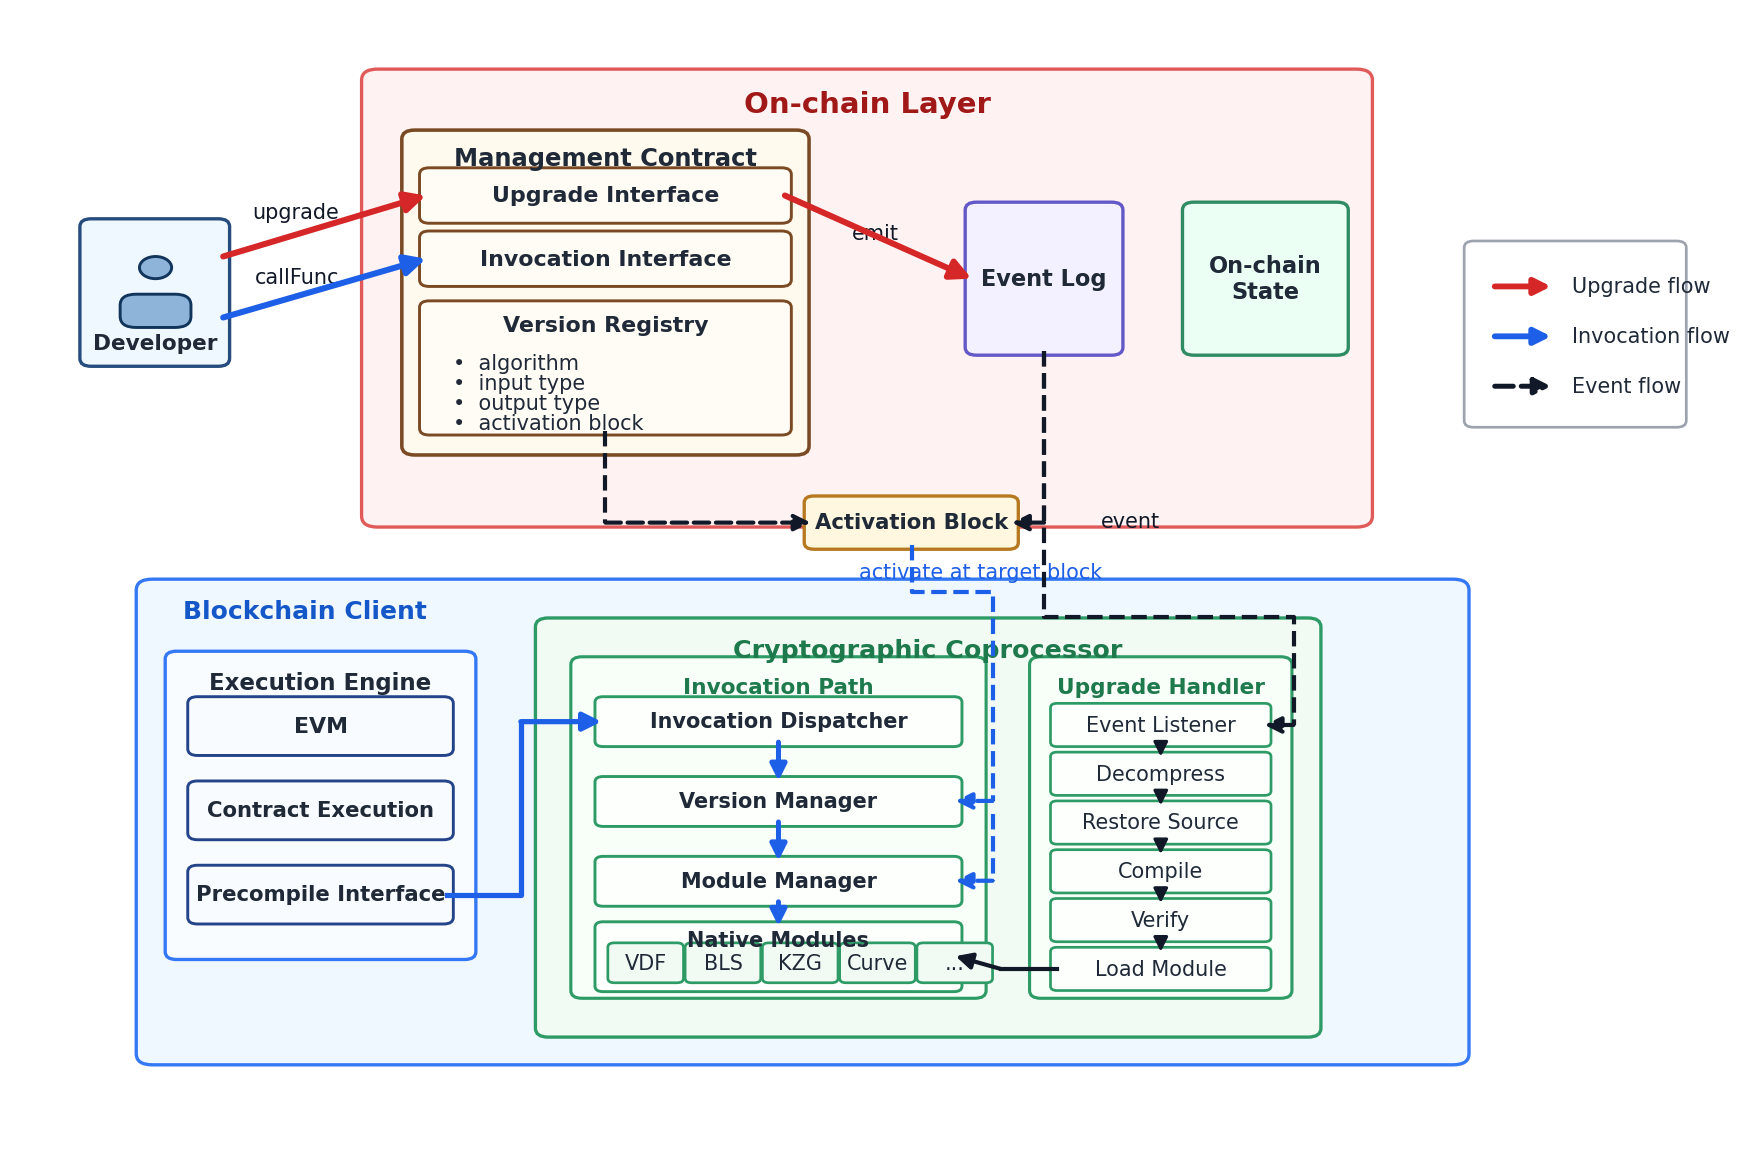
\includegraphics[width=\textwidth]{../image/overview.png}
\caption{Overall architecture of the Cryptographic Coprocessor. The on-chain layer publishes upgrade proposals, stores version metadata, and emits events. The client layer separates invocation dispatch from upgrade preparation: the execution engine routes calls into the coprocessor, while the upgrade handler restores, compiles, verifies, and loads Native modules. The Activation Block determines when a prepared module becomes active.}
\label{fig:overview}
\end{figure}

The architecture contains four main components. First, the Management Contract, implemented as CodeStorage in the prototype, is the EVM-facing interface used by contracts and upgrade transactions. It provides \texttt{callFunc} for algorithm invocation and upload functions for publishing algorithm metadata. Second, the EVM integration layer recognizes calls to the CodeStorage address and dispatches them to the coprocessor boundary rather than to ordinary contract bytecode. Third, the coprocessor runtime manages ABI decoding, gas metadata, algorithm lookup, and version selection. Fourth, the upgrade handler maintains the node-local workspace that stores decoded source files, compiled shared objects, and persistent algorithm metadata. These components define a small client-side boundary around cryptographic algorithms while leaving unrelated EVM execution semantics outside the upgrade mechanism.

\subsection{Invocation Abstraction}\label{sec3.2}
The invocation abstraction separates the contract-facing interface from the Native implementation that performs the cryptographic computation. From the contract side, an algorithm call is expressed as a stable ABI request, \texttt{callFunc(name,input)}, where \texttt{name} identifies the algorithm and \texttt{input} carries ABI-encoded parameters. The contract does not depend on the location of the compiled artifact, the internal Go function, or the client-side loading state. This is the main abstraction boundary: contracts bind to an EVM-visible interface, whereas the client binds that interface to a local implementation chosen at execution time.

Inside the client, the coprocessor parses the CodeStorage calldata, normalizes the algorithm name, retrieves the algorithm metadata, and decodes the input according to the stored input type list. It then resolves the implementation. Built-in cryptographic routines can be called through the internal registry, while dynamically upgraded algorithms are invoked through a loaded plugin whose exported symbol matches the normalized algorithm name. After the Native function returns, the coprocessor re-encodes the result according to the stored output type list and returns the bytes to the EVM. Gas is obtained from the corresponding algorithm metadata and charged through the EVM call path before execution proceeds.

This abstraction has two consequences. First, replacing an algorithm implementation does not require changing the contract-facing call shape, as long as the metadata and ABI-level input-output contract remain compatible with the intended use. Second, the EVM integration does not need to understand the internals of every cryptographic algorithm. It only needs a stable dispatch boundary, a gas query, and a deterministic return value for the selected algorithm version. The mechanism therefore decouples contract-facing cryptographic algorithms from their Native implementations, rather than attempting to make arbitrary client logic dynamically replaceable.

\subsection{Dynamic Upgrade}\label{sec3.3}
Dynamic upgrade starts from an on-chain upgrade proposal. In the versioned path, the proposal is submitted through \texttt{uploadCodeVersion}, carrying the algorithm name, version number, encoded source artifact, gas value, ABI input and output type descriptions, and the Activation Block. During transaction execution, CodeStorage validates the metadata, stores it in the chain state, and emits a \texttt{codeVersionUploaded} event. Crucially, this EVM path does not compile the source artifact or open the plugin. It only records the authoritative metadata and publishes the event that clients can observe.

Each client runs an Event Listener for CodeStorage upgrade events. When the listener observes a versioned upgrade event, it queries the authoritative metadata from CodeStorage, checks that the event and the stored metadata agree on the version and Activation Block, and delegates the work to the activation service. The activation service decodes the uploaded source into the local plugin workspace, compiles it with \texttt{go build -buildmode=plugin}, publishes the resulting shared object, and asks the plugin loader to verify that the expected exported symbol exists. Only after these steps succeed is the version recorded locally as a prepared version.

This workflow separates on-chain coordination from node-local preparation. The chain provides a single upgrade proposal and a stable metadata source, while each node independently performs compilation and loading according to its local environment. A preparation failure is local to the node: it does not roll back the already executed upgrade transaction, and it must not be interpreted as successful local activation. This separation is the basis for asynchronous upgrade preparation, and it is also the reason the upgrade transaction itself is not required to wait for plugin compilation.

\subsection{Deterministic Activation}\label{sec3.4}
Asynchronous preparation creates a consistency problem if nodes switch algorithm versions as soon as their local plugin is ready. Two nodes may observe the same chain but finish compilation at different physical times; if readiness time determined the active version, the same contract call could execute different Native implementations. The coprocessor therefore separates preparation time from activation time. The upgrade proposal includes an Activation Block, and the client selects algorithm versions by block height rather than by local completion time.

For a call executed at block height \(H\), the version selector chooses the prepared version whose Activation Block is not greater than \(H\), preferring the newest applicable version when multiple versions are available. Before the Activation Block, calls continue to resolve to the previous applicable version. At and after the Activation Block, ready nodes resolve the call to the new version. This rule makes activation deterministic with respect to chain height: given the same chain view, metadata, and prepared artifacts, nodes use the same version-selection rule for the same block height.

The design also defines a failure boundary. If a node reaches the Activation Block but has not prepared the target version required for that height, it must not silently fall back to the obsolete implementation for calls that require the new semantics. In the prototype, the runtime checks whether the selected version is locally prepared and returns an execution error if the required version is missing. This behavior is a design constraint rather than a universal consistency proof: it prevents a locally unprepared node from producing an apparently valid result with the wrong algorithm, but it does not by itself prove correctness under every network, scheduler, or fault scenario.

\section{Evaluation}\label{sec4}

The evaluation asks whether the proposed coprocessor can be used as a practical execution path for upgradable contract-facing cryptographic algorithms. We focus on three questions that correspond to the design goals in Section~\ref{sec3}: how much observable latency and upload cost the upgrade workflow introduces, whether dynamically loaded algorithms retain Native execution efficiency after activation, and whether the Activation Block mechanism preserves consistent version selection and outputs across nodes under the evaluated private-chain scenarios.

\subsection{Overview}\label{sec4.1}
We implemented the prototype by extending Geth with the CodeStorage interface, the client-side Cryptographic Coprocessor, and the event-driven upgrade handler. The experiments were run on a Geth-based private chain on Ubuntu 24.04. For the multi-node experiments, we used a five-node Clique network with one signer and four observer nodes, a block period of 5 s, and network identifier 11223344. The current experiment ledger does not record the host CPU, memory, storage device, or exact prototype commit; these metadata remain TODO for reproducibility reporting.

The evaluation covers seven algorithms: Add, Sha256, Blake2bSum256, Pbkdf2Sha256, Dh2048Secret, PedersenCommit, and SchnorrVerify. Add is a non-cryptographic baseline, whereas the remaining algorithms exercise hash functions, password-based key derivation, key exchange, commitments, and signature verification. For upgrade latency, the completion criterion is not an internal ``ready'' flag. A node is counted as complete only when its RPC endpoint returns the expected output from \texttt{CodeStorage.callFunc}. For execution efficiency, we compare three paths after setup has completed: Upgrade, which invokes a dynamically loaded Native module through CodeStorage; Precompile, which invokes a client-native Precompiled Contract; and Contract, which executes a Solidity contract implementation. We report \texttt{eth\_call} latency and \texttt{gasEstimate}, where the latter is obtained from \texttt{eth\_estimateGas} and should not be interpreted as receipt \texttt{gasUsed}. For state consistency, we evaluate scheduled and immediate activation modes on the same five-node private chain and check version, output, receipt/event, and chain-view consistency.

\subsection{Upgrade Latency and Upload Cost}\label{sec4.2}
The upgrade-latency experiment measured the control-plane time from submitting an upgrade transaction to the point at which all five target nodes could call the uploaded algorithm successfully. This measurement is intentionally end-to-end and externally observable. It includes RPC round trips and polling intervals, and therefore should not be read as a precise decomposition of the internal compilation time of each node.

Figure~\ref{fig:lab1-upgrade-latency} shows the latency breakdown for the seven algorithms. Across the five-node Clique experiments, the total submit-to-all-complete latency ranged from 20.35 s for Blake2bSum256 to 31.41 s for Dh2048Secret. The sender observed a successful transaction receipt after 5.40--7.87 s, whereas the event-to-all-complete interval accounted for 13.00--23.54 s. In these runs, the event was confirmed from the successful upgrade transaction receipt, so the receipt-to-event interval was effectively zero at the controller. The node-level completion times were tightly clustered in the fault-free local network: the largest observed spread between the fastest and slowest node for the same algorithm was 0.727 s. These results support the intended separation between on-chain upgrade publication and node-local preparation. The upgrade transaction completed before all nodes became callable, indicating that source restoration, plugin compilation, symbol verification, and loading were outside the EVM execution path of that transaction.

\begin{figure}[H]
\centering
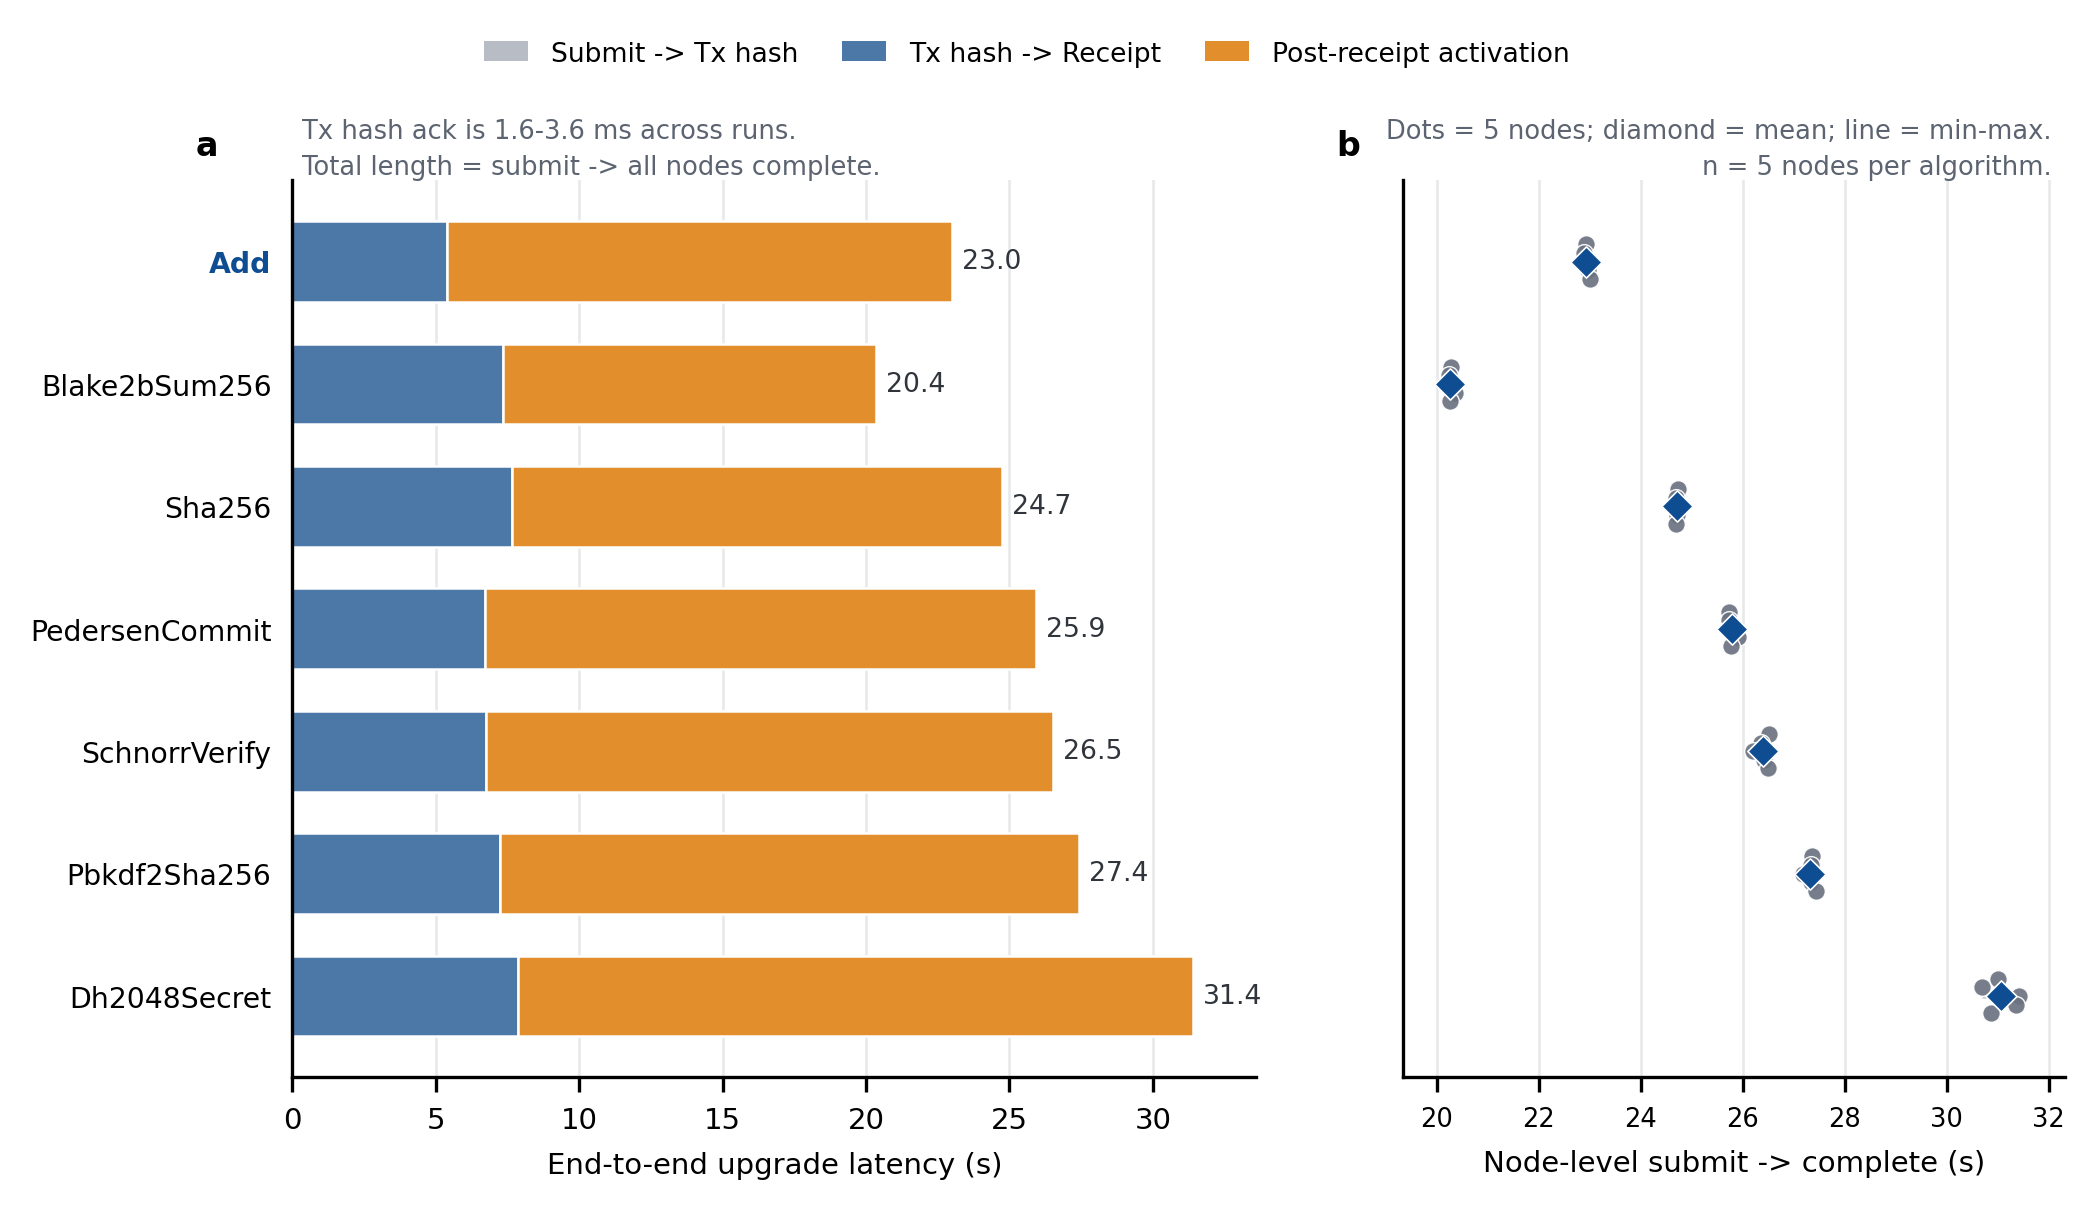
\includegraphics[width=\textwidth]{../image/lab1-upgrade-latency-availability/lab1_upgrade_latency_5nodes.pdf}
\caption{Upgrade latency in the five-node Clique private chain. The measurement starts when the controller submits the upgrade transaction and ends when every target node can return the expected output through \texttt{CodeStorage.callFunc}. The event-to-all-complete interval includes RPC polling and node-local preparation, not only internal plugin compilation.}
\label{fig:lab1-upgrade-latency}
\end{figure}

We also measured the upload cost of the event-bearing upgrade transaction and compared it with Solidity contract deployment for Add and Blake2bSum256 (Figure~\ref{fig:lab1-deployment-cost}). This auxiliary experiment measures the total upload transaction cost; it does not isolate the gas of the event log alone from storage and calldata costs. For Add, the upgrade upload used 85,612 gas, compared with 60,918 gas for the minimal Solidity deployment, and the mean receipt latency was 1.71 s versus 1.01 s. For Blake2bSum256, the upgrade upload used 87,180 gas, whereas the Solidity deployment used 852,059 gas; the corresponding mean receipt latencies were 1.71 s and 1.01 s. Precompiled Contracts have no deployment transaction in this comparison because they are already built into the client. The result shows a cost trade-off: the upgrade path introduces a separate upload transaction and event-driven preparation, but for a code-heavy algorithm such as Blake2bSum256 it can avoid the large deployment gas incurred by a Solidity implementation. Because this auxiliary cost experiment covers only Add and Blake2bSum256, we do not generalize the deployment-cost trend to all algorithms.

\begin{figure}[H]
\centering
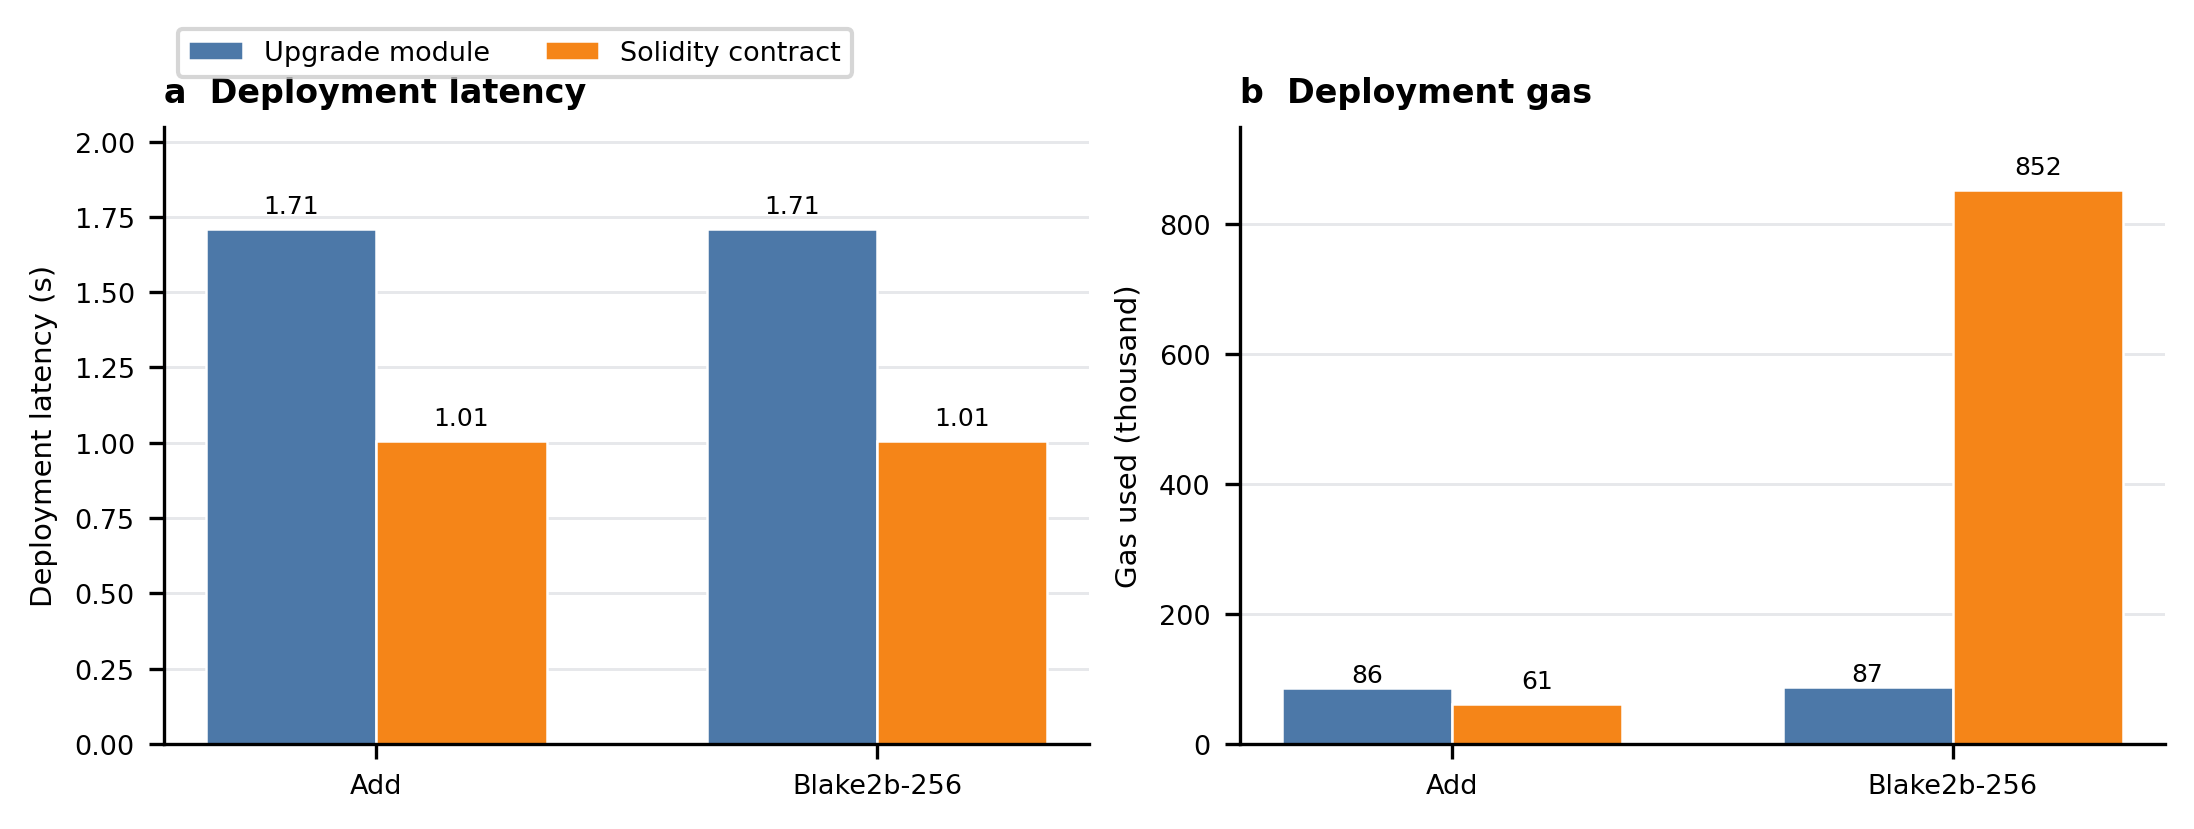
\includegraphics[width=\textwidth]{../image/lab1-upgrade-latency-availability/lab1_deployment_upgrade_cost.pdf}
\caption{Upload and deployment cost for the auxiliary Lab1 cost experiment. The upgrade path uses \texttt{CodeStorage.uploadCode} and emits an upgrade event, whereas the Contract path deploys a Solidity implementation. The figure reports total transaction-level setup cost, not an isolated event-log gas component.}
\label{fig:lab1-deployment-cost}
\end{figure}

\subsection{Execution Efficiency}\label{sec4.3}
The execution-efficiency experiment evaluated whether the dynamic upgrade mechanism adds substantial overhead after an algorithm has already been prepared. Each algorithm was measured with 10 warm-up calls and 100 formal \texttt{eth\_call} samples for each implementation path. The comparison therefore concerns steady-state invocation cost, not setup or upload latency.

Figure~\ref{fig:lab2-execution-latency} compares mean \texttt{eth\_call} latency across Upgrade, Precompile, and Contract paths. The Upgrade path remained close to the Precompile path for the evaluated algorithms: mean latency ranged from 0.894 to 2.663 ms for Upgrade and from 0.860 to 3.235 ms for Precompile. For simple operations such as Add and Sha256, all three paths were near the millisecond level. For more computationally intensive algorithms, the Native paths were more clearly separated from Solidity execution. For example, PedersenCommit took 1.245 ms through Upgrade and 1.079 ms through Precompile, compared with 5.514 ms through Contract; SchnorrVerify took 2.663 ms through Upgrade and 3.235 ms through Precompile, compared with 8.017 ms through Contract. These observations support the main performance claim in a bounded form: dynamically loaded algorithms execute as Native code and retain performance comparable to client-native Precompiled Contracts under this benchmark, without implying that the Upgrade path is universally faster.

\begin{figure}[H]
\centering
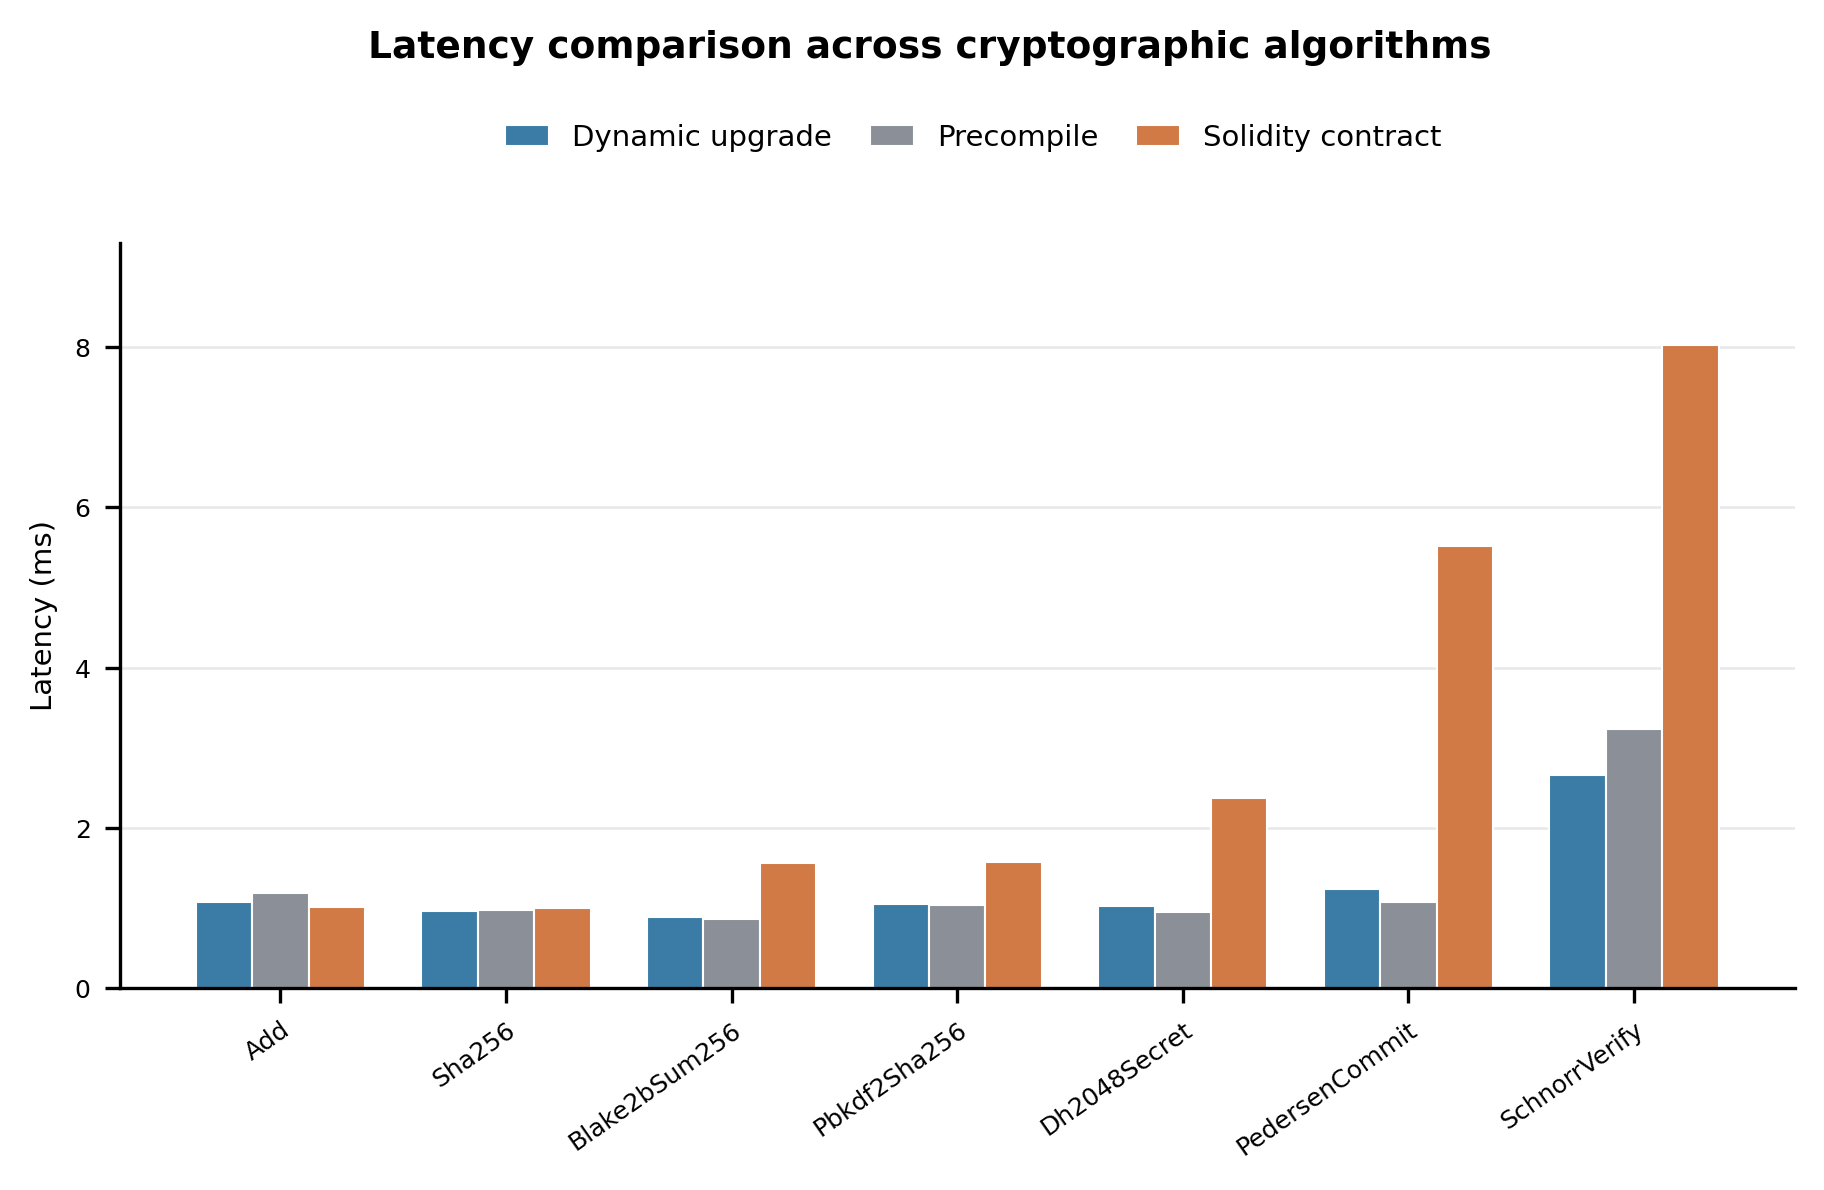
\includegraphics[width=\textwidth]{../image/lab2-execution-efficiency/lab2_execution_efficiency_latency.pdf}
\caption{Execution latency after setup. Upgrade invokes a dynamically loaded Native module through CodeStorage, Precompile invokes a client-native Precompiled Contract, and Contract executes a Solidity implementation. Latency is measured by repeated \texttt{eth\_call} after warm-up.}
\label{fig:lab2-execution-latency}
\end{figure}

Figure~\ref{fig:lab2-gas-estimate} reports \texttt{gasEstimate} for the same calls. Upgrade and Precompile had similar gas estimates under the prototype pricing model for the evaluated Native paths. For Sha256, the estimates were 25,801 gas for Upgrade and 25,156 gas for Precompile; for Blake2bSum256, the same two values were observed. For complex Solidity implementations, the Contract path incurred substantially larger estimates: PedersenCommit required 868,629 gas compared with 225,695 gas for Upgrade, and SchnorrVerify required 9,527,269 gas compared with 229,437 gas for Upgrade. These gas numbers should be interpreted only as the current prototype's pricing results from \texttt{eth\_estimateGas}. They do not prove that the proposed architecture has inherently lower economic cost than official Ethereum precompile pricing, and they are not receipt-level \texttt{gasUsed} measurements.

\begin{figure}[H]
\centering
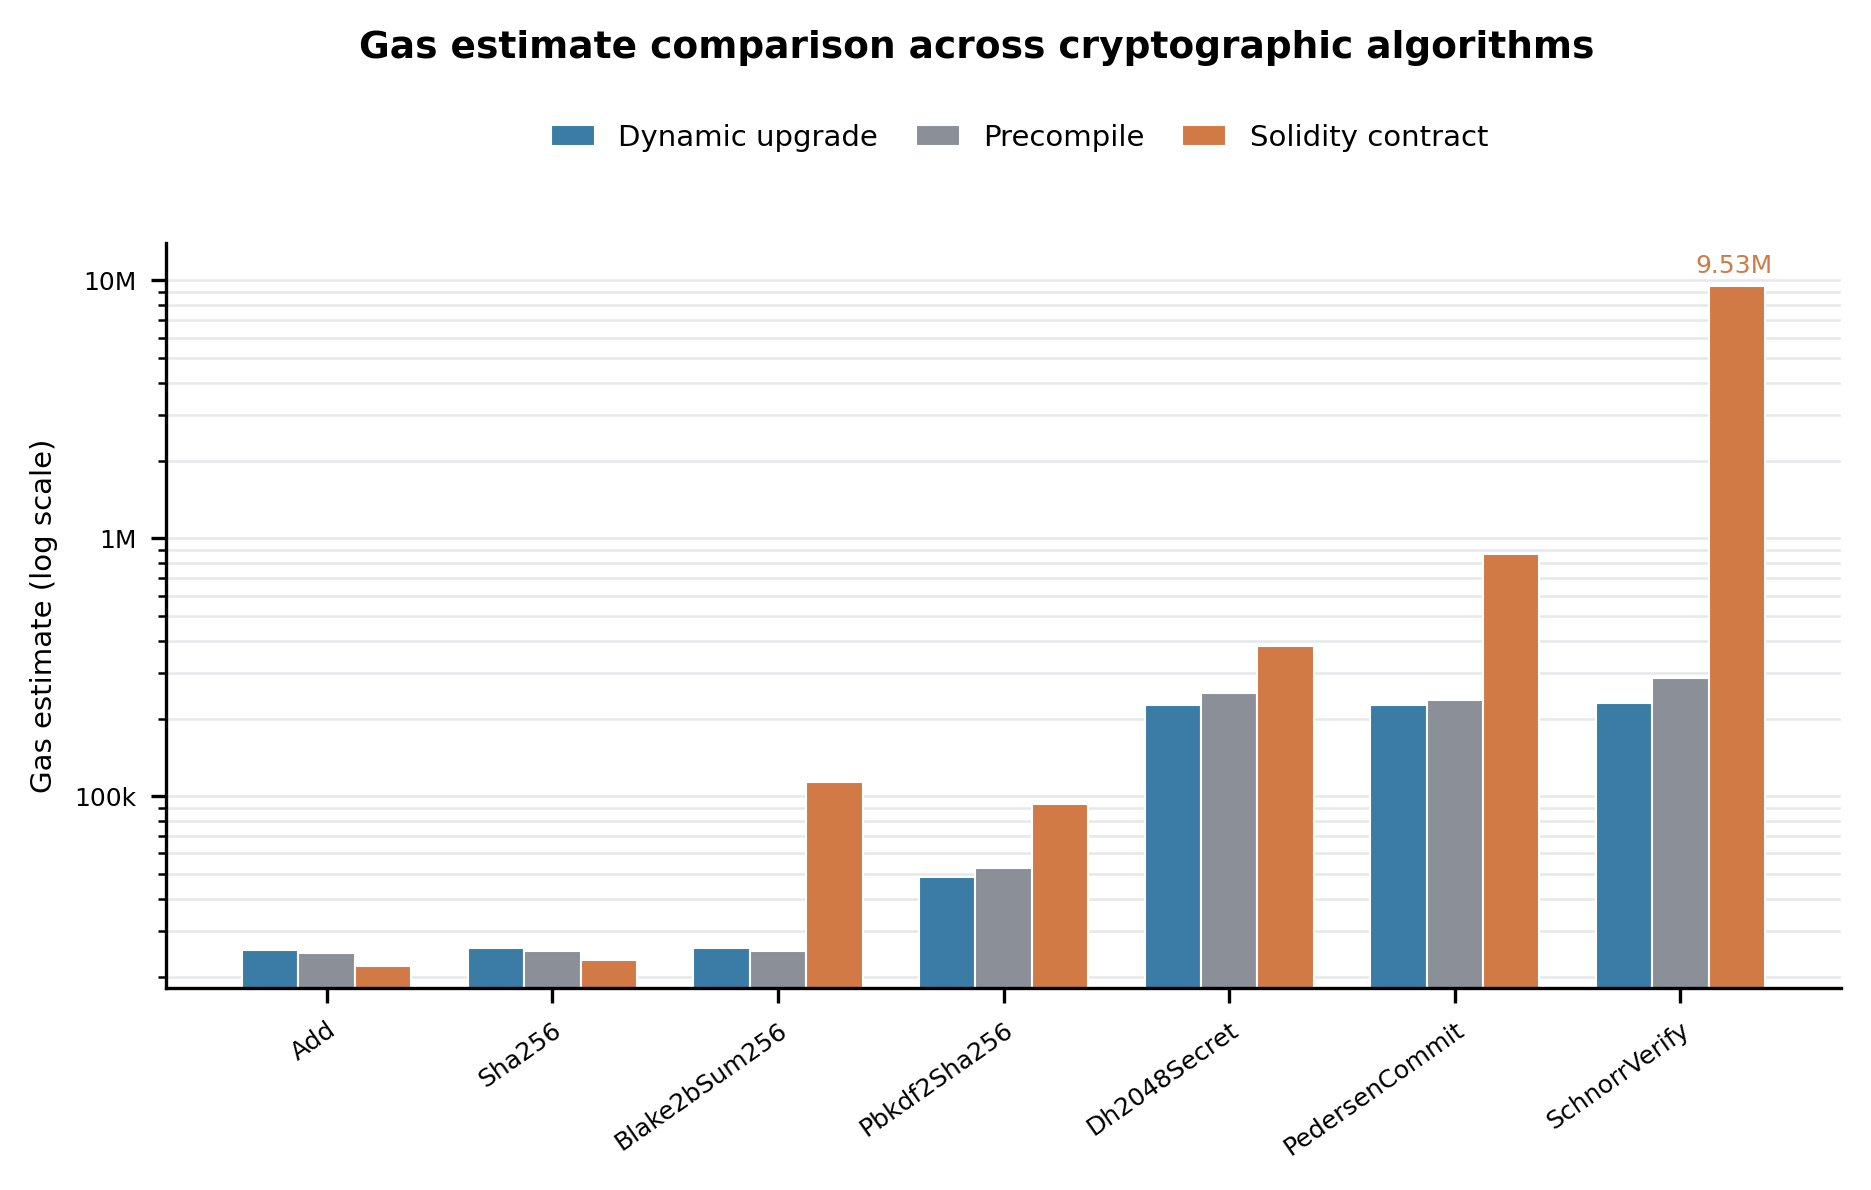
\includegraphics[width=\textwidth]{../image/lab2-execution-efficiency/lab2_execution_efficiency_gas_estimate.pdf}
\caption{Gas estimates for steady-state algorithm invocation. Values are obtained from \texttt{eth\_estimateGas}; they reflect the prototype pricing model and are not receipt \texttt{gasUsed}.}
\label{fig:lab2-gas-estimate}
\end{figure}

\subsection{State Consistency}\label{sec4.4}
The state-consistency experiment evaluated whether version activation remains deterministic across nodes after an upgrade transaction is included in the private chain. The experiment used the same five-node Clique setting and ran four rounds in total: two scheduled rounds and two immediate rounds. Both modes used an \texttt{activationBlock}; the immediate mode set the activation block to the block in which the upgrade became effective, and should not be interpreted as a baseline without deterministic activation.

Figure~\ref{fig:lab3-state-consistency} summarizes the consistency checks. All four rounds passed. In the scheduled mode, nodes returned the old-version output 200 at \(\texttt{activationBlock}-1\) and the new-version output 205 at \(\texttt{activationBlock}\). In the immediate mode, nodes returned the new-version output 205 from the effective upgrade block. For each sampled canonical block, all nodes agreed on block hash, receipt block hash, version, Activation Block, metadata hash, and algorithm output. These observations support version consistency, execution consistency, and chain-view consistency under the evaluated fault-free private-chain scenarios.

\begin{figure}[H]
\centering
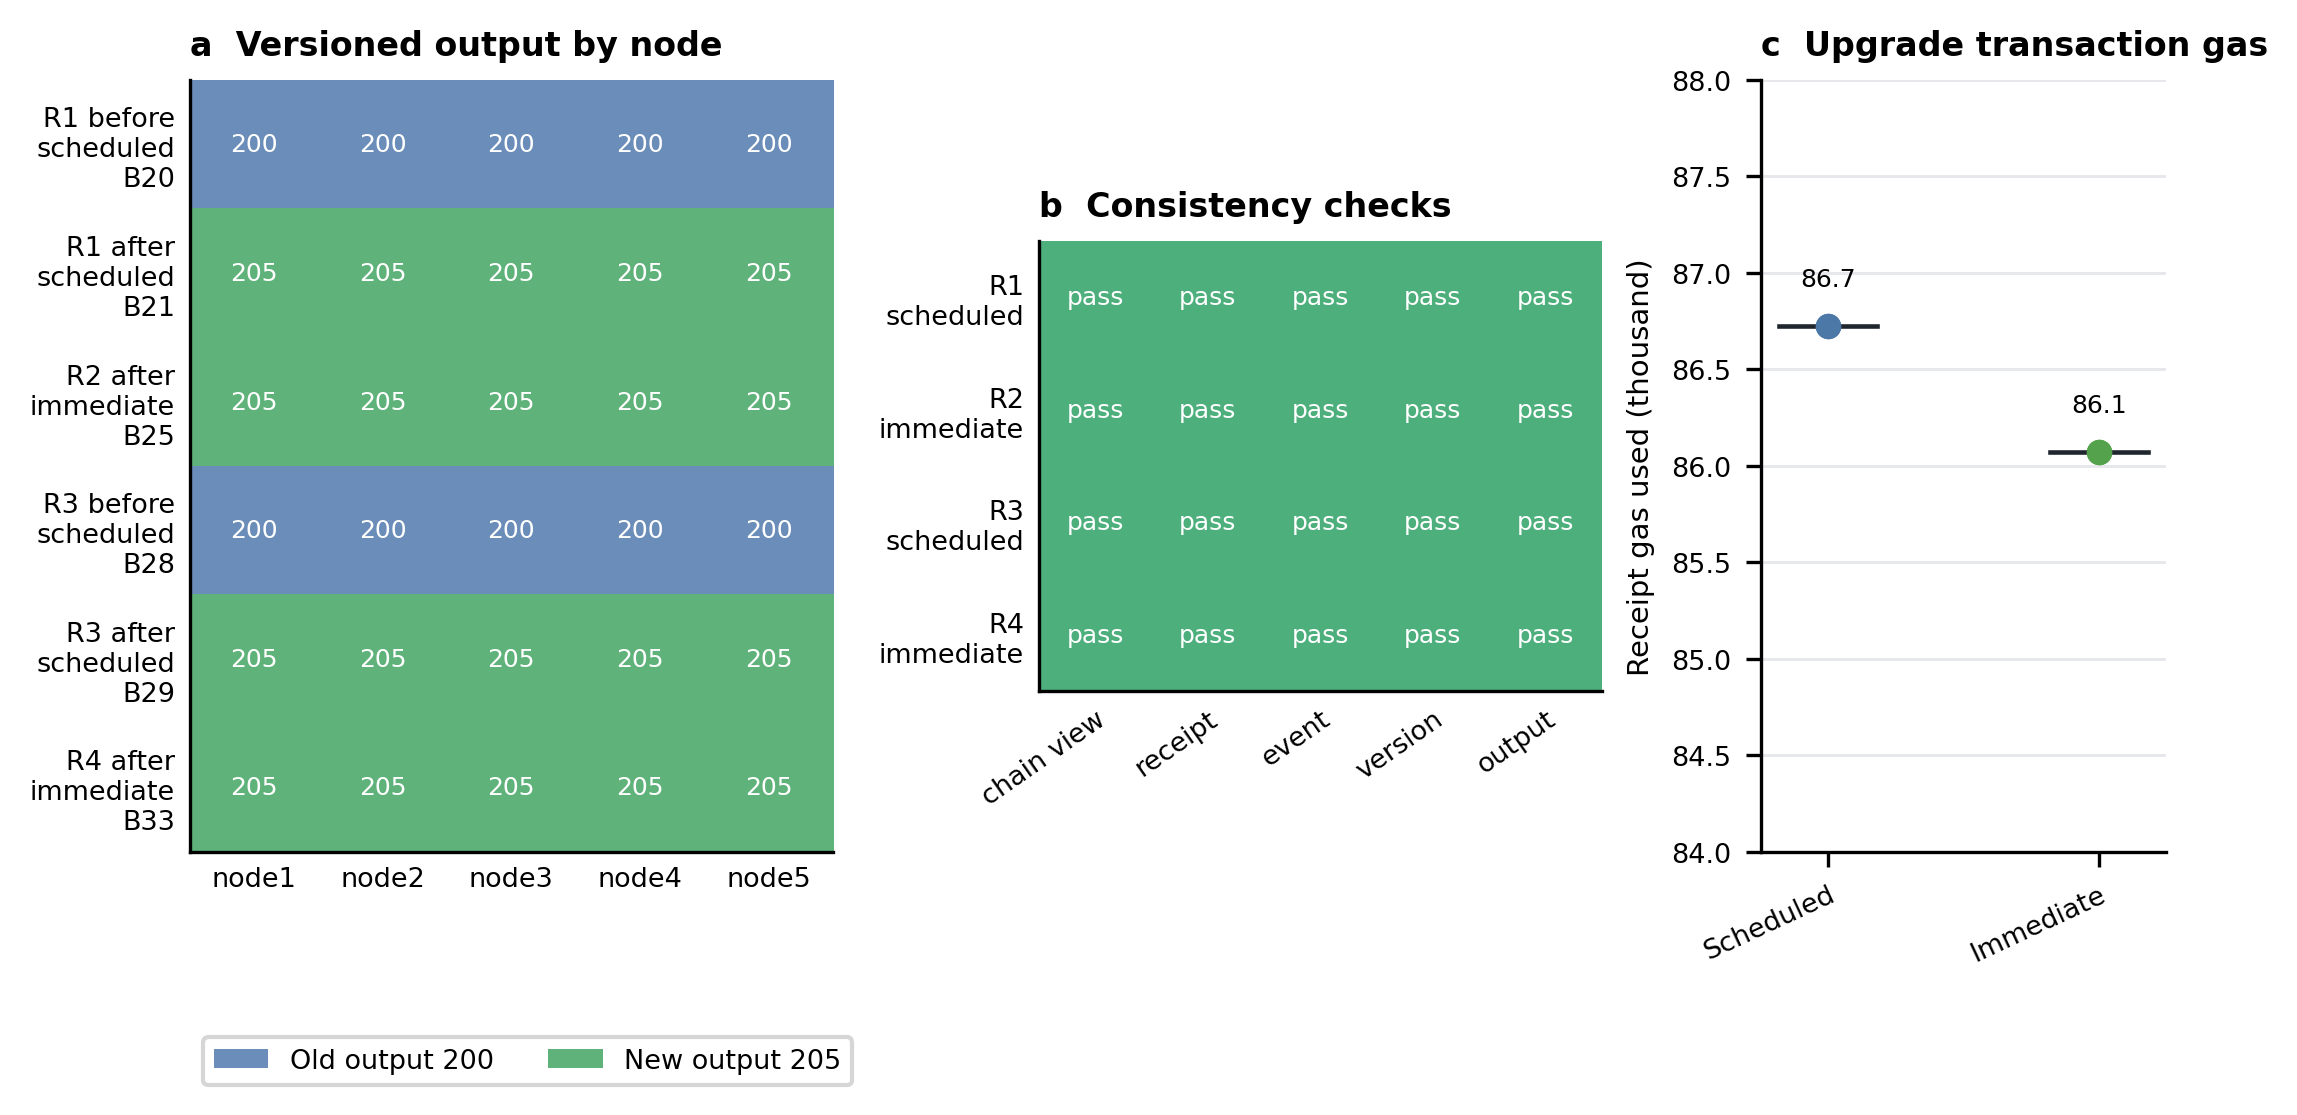
\includegraphics[width=\textwidth]{../image/lab3-state-consistency/lab3_upgrade_state_consistency_5nodes.pdf}
\caption{State-consistency checks for scheduled and immediate activation. The experiment verifies version selection, output agreement, receipt visibility, metadata hash agreement, and chain-view consistency across five Clique nodes.}
\label{fig:lab3-state-consistency}
\end{figure}

The current consistency result is deliberately bounded. The formal Lab3 data do not contain \texttt{stateRoot}, and the experiment did not inject an unprepared node at the Activation Block. Therefore, the result should not be described as a formal consensus-safety proof, a universal guarantee for arbitrary network sizes, or an experimental validation of fail-stop behavior. Within the evaluated scenario, however, the data show that the Activation Block separated asynchronous preparation from deterministic execution: local preparation time did not define the active algorithm version, while the chain height did.

\section{Related Work}\label{sec5}

This work is related to two lines of research: software upgrade mechanisms that change running systems without stopping the whole service, and blockchain upgrade mechanisms that must additionally preserve deterministic execution and verifiable history. We organize the discussion by mechanism rather than by publication date, because the central question is not whether code can be replaced, but where the upgrade boundary is placed and how consistency is preserved.

\subsection{Software Upgrade Mechanisms}\label{sec5.1}
Dynamic software update (DSU) studies how a running program can change code or components while preserving service availability. KylinX uses page-level and library-level dynamic mapping to support runtime library replacement in a Unikernel-like virtualization setting while retaining strong isolation \cite{zhang2018kylinx}. Mvedsua combines dynamic software update with multi-version execution so that old and new versions can run together during an update and tolerate update-time errors \cite{pina2019mvedsua}. PYLIVE exploits Python's interpreted execution model to support portable on-the-fly code changes for Python-based online services \cite{huang2021pylive}. Ajmani et al. proposed modular software upgrades for distributed systems by using a central upgrade service to coordinate versioned components and storage \cite{ajmani2006modular}. Baresi et al. linked dynamic dependencies with version consistency so that distributed components can be updated in windows that preserve cross-component compatibility \cite{baresi2017versionConsistency}.

These systems establish useful upgrade concepts, including dynamic loading, multi-version execution, and version-consistent distributed update. However, they do not directly address the blockchain requirement that independently executing nodes must choose the same semantics for the same block height. Our work therefore borrows the general idea of runtime replacement but moves the consistency boundary to the chain: the upgrade proposal is coordinated on chain, local preparation is asynchronous, and activation is determined by the Activation Block rather than by local readiness time.

\subsection{Blockchain Upgrade Mechanisms}\label{sec5.2}
Blockchain upgrades must preserve not only service continuity but also transaction verifiability, replayability, and consensus-compatible state evolution. Cardano's hard-fork-combinator documentation describes a mechanism for switching between protocol eras at a designated upgrade point while keeping the chain history under a unified abstraction \cite{cardanoHardForkCombinator}. Cardano's evolution documentation further presents hard forks as planned protocol transitions that require compatibility across ledger and consensus rules \cite{cardanoEvolution}. Ciampi et al. studied updatable blockchains by translating blocks between old and new chains so that hard-fork-style upgrades can remain synchronized across versions \cite{ciampi2020updatable}. Zindros proposed a soft-fork-based method for upgrading blockchain macroeconomic policy by abstracting policy parameters and algorithms into smart contracts \cite{zindros2021softPower}. Phoenix embeds upgrade code in blockchain transactions and uses just-in-time compilation to build a live-upgradable blockchain client \cite{wang2023phoenix}. Polkadot uses on-chain governance and a WASM-based runtime so that approved runtime logic can be stored on chain and adopted by nodes during synchronization \cite{polkadotRuntimeUpgrades}. EVMPatch automatically patches vulnerable Ethereum smart contracts through bytecode rewriting, historical-transaction testing, and proxy-based deployment \cite{rodler2021evmpatch}.

These blockchain mechanisms cover protocol-era transitions, hard-fork synchronization, policy-level soft forks, client-wide live update, runtime replacement, and contract patching. They differ from our target in both scope and execution boundary. Protocol-level mechanisms such as Cardano and Polkadot update broad chain logic and require a runtime or protocol abstraction that is larger than a single class of cryptographic functions. Client-level mechanisms such as Phoenix update executable client logic but may introduce repeated retrieval and compilation costs when upgrade code is interpreted or compiled from chain storage. Contract-level mechanisms such as EVMPatch repair deployed contract bytecode but do not replace client-native cryptographic algorithms behind a stable contract-facing interface. In contrast, the Cryptographic Coprocessor targets contract-facing cryptographic algorithms specifically: the contract interface remains stable, the Native implementation is prepared locally as a plugin, and deterministic activation is tied to an on-chain Activation Block.

\section{Conclusion}\label{sec6}

This paper addressed the upgrade problem of contract-facing cryptographic algorithms by proposing a Cryptographic Coprocessor architecture for smart-contract-enabled blockchain clients. The central idea is to separate the stable EVM-facing invocation interface from the client-side Native implementation, so that smart contracts can keep the same call boundary while the client manages cryptographic algorithms as replaceable modules. The design combines on-chain upgrade coordination, off-chain asynchronous preparation, dynamic plugin loading, and block-height-based deterministic activation. In this way, cryptographic algorithm updates can be prepared while the client process continues to run and do not need to follow the same path as rebuilding and redeploying the whole client software, which lowers the operational cost of cryptographic evolution and provides a practical basis for responding to long-term security migration needs, including post-quantum migration.

The prototype and experiments support this design under the evaluated private-chain scenarios. The upgrade-latency experiment showed that an upgrade transaction can record metadata and emit an event before all nodes finish local preparation, indicating that source restoration, compilation, verification, and loading are outside the EVM execution critical path of that transaction. The execution-efficiency experiment showed that dynamically loaded Native algorithms remain close to Precompiled Contract execution for the evaluated algorithms while avoiding the high Solidity/EVM overhead observed for complex cryptographic computations. The state-consistency experiment showed that scheduled and immediate activation modes preserved version, output, receipt/event, and chain-view consistency across the evaluated five-node Clique private chain. These results do not constitute a proof of uninterrupted service availability or universal consensus safety, but they demonstrate that asynchronous preparation and deterministic activation can be combined without changing the contract-facing interface.

Several research problems remain open. First, future work should design a gas pricing mechanism for dynamically upgraded cryptographic algorithms that reflects execution cost, storage cost, calldata cost, and data availability pressure, rather than relying only on manually assigned Native pricing rules. Second, the upgrade channel itself must be hardened against denial-of-service (DoS) attacks and data availability saturation attacks, because an attacker could submit large or expensive upgrade artifacts to consume client compilation, storage, or propagation resources. Third, compatibility across algorithm versions should be strengthened through explicit ABI-version constraints, artifact metadata, deprecation policies, and checks that prevent unsafe interface changes. Finally, broader implementation-language compatibility is needed: the current prototype uses Go plugins, whereas a production system may require sandboxed WebAssembly, C/C++ shared libraries, Rust components, or other language runtimes with deterministic invocation and verifiable build metadata. Addressing these problems would move the coprocessor from a prototype mechanism toward a more general upgrade substrate for blockchain cryptographic services.
%\section{Results}\label{sec2}
%
%Sample body text. Sample body text. Sample body text. Sample body text. Sample body text. Sample body text. Sample body text. Sample body text.
%
%\section{This is an example for first level head---section head}\label{sec3}
%
%\subsection{This is an example for second level head---subsection head}\label{subsec2}
%
%\subsubsection{This is an example for third level head---subsubsection head}\label{subsubsec2}
%
%Sample body text. Sample body text. Sample body text. Sample body text. Sample body text. Sample body text. Sample body text. Sample body text. 
%
%\section{Equations}\label{sec4}
%
%Equations in \LaTeX\ can either be inline or on-a-line by itself (``display equations''). For
%inline equations use the \verb+$...$+ commands. E.g.: The equation
%$H\psi = E \psi$ is written via the command \verb+$H \psi = E \psi$+.
%
%For display equations (with auto generated equation numbers)
%one can use the equation or align environments:
%\begin{equation}
%\|\tilde{X}(k)\|^2 \leq\frac{\sum\limits_{i=1}^{p}\left\|\tilde{Y}_i(k)\right\|^2+\sum\limits_{j=1}^{q}\left\|\tilde{Z}_j(k)\right\|^2 }{p+q}.\label{eq1}
%\end{equation}
%where,
%\begin{align}
%D_\mu &=  \partial_\mu - ig \frac{\lambda^a}{2} A^a_\mu \nonumber \\
%F^a_{\mu\nu} &= \partial_\mu A^a_\nu - \partial_\nu A^a_\mu + g f^{abc} A^b_\mu A^a_\nu \label{eq2}
%\end{align}
%Notice the use of \verb+\nonumber+ in the align environment at the end
%of each line, except the last, so as not to produce equation numbers on
%lines where no equation numbers are required. The \verb+\label{}+ command
%should only be used at the last line of an align environment where
%\verb+\nonumber+ is not used.
%\begin{equation}
%Y_\infty = \left( \frac{m}{\textrm{GeV}} \right)^{-3}
%    \left[ 1 + \frac{3 \ln(m/\textrm{GeV})}{15}
%    + \frac{\ln(c_2/5)}{15} \right]
%\end{equation}
%The class file also supports the use of \verb+\mathbb{}+, \verb+\mathscr{}+ and
%\verb+\mathcal{}+ commands. As such \verb+\mathbb{R}+, \verb+\mathscr{R}+
%and \verb+\mathcal{R}+ produces $\mathbb{R}$, $\mathscr{R}$ and $\mathcal{R}$
%respectively (refer Subsubsection~\ref{subsubsec2}).
%
%\section{Tables}\label{sec5}
%
%Tables can be inserted via the normal table and tabular environment. To put
%footnotes inside tables you should use \verb+\footnotetext[]{...}+ tag.
%The footnote appears just below the table itself (refer Tables~\ref{tab1} and \ref{tab2}). 
%For the corresponding footnotemark use \verb+\footnotemark[...]+
%
%\begin{table}[h]
%\caption{Caption text}\label{tab1}%
%\begin{tabular}{@{}llll@{}}
%\toprule
%Column 1 & Column 2  & Column 3 & Column 4\\
%\midrule
%row 1    & data 1   & data 2  & data 3  \\
%row 2    & data 4   & data 5\footnotemark[1]  & data 6  \\
%row 3    & data 7   & data 8  & data 9\footnotemark[2]  \\
%\botrule
%\end{tabular}
%\footnotetext{Source: This is an example of table footnote. This is an example of table footnote.}
%\footnotetext[1]{Example for a first table footnote. This is an example of table footnote.}
%\footnotetext[2]{Example for a second table footnote. This is an example of table footnote.}
%\end{table}
%
%\noindent
%The input format for the above table is as follows:
%
%%%=============================================%%
%%% For presentation purpose, we have included  %%
%%% \bigskip command. Please ignore this.       %%
%%%=============================================%%
%\bigskip
%\begin{verbatim}
%\begin{table}[<placement-specifier>]
%\caption{<table-caption>}\label{<table-label>}%
%\begin{tabular}{@{}llll@{}}
%\toprule
%Column 1 & Column 2 & Column 3 & Column 4\\
%\midrule
%row 1 & data 1 & data 2	 & data 3 \\
%row 2 & data 4 & data 5\footnotemark[1] & data 6 \\
%row 3 & data 7 & data 8	 & data 9\footnotemark[2]\\
%\botrule
%\end{tabular}
%\footnotetext{Source: This is an example of table footnote. 
%This is an example of table footnote.}
%\footnotetext[1]{Example for a first table footnote.
%This is an example of table footnote.}
%\footnotetext[2]{Example for a second table footnote. 
%This is an example of table footnote.}
%\end{table}
%\end{verbatim}
%\bigskip
%%%=============================================%%
%%% For presentation purpose, we have included  %%
%%% \bigskip command. Please ignore this.       %%
%%%=============================================%%
%
%\begin{table}[h]
%\caption{Example of a lengthy table which is set to full textwidth}\label{tab2}
%\begin{tabular*}{\textwidth}{@{\extracolsep\fill}lcccccc}
%\toprule%
%& \multicolumn{3}{@{}c@{}}{Element 1\footnotemark[1]} & \multicolumn{3}{@{}c@{}}{Element 2\footnotemark[2]} \\\cmidrule{2-4}\cmidrule{5-7}%
%Project & Energy & $\sigma_{calc}$ & $\sigma_{expt}$ & Energy & $\sigma_{calc}$ & $\sigma_{expt}$ \\
%\midrule
%Element 3  & 990 A & 1168 & $1547\pm12$ & 780 A & 1166 & $1239\pm100$\\
%Element 4  & 500 A & 961  & $922\pm10$  & 900 A & 1268 & $1092\pm40$\\
%\botrule
%\end{tabular*}
%\footnotetext{Note: This is an example of table footnote. This is an example of table footnote this is an example of table footnote this is an example of~table footnote this is an example of table footnote.}
%\footnotetext[1]{Example for a first table footnote.}
%\footnotetext[2]{Example for a second table footnote.}
%\end{table}
%
%In case of double column layout, tables which do not fit in single column width should be set to full text width. For this, you need to use \verb+\begin{table*}+ \verb+...+ \verb+\end{table*}+ instead of \verb+\begin{table}+ \verb+...+ \verb+\end{table}+ environment. Lengthy tables which do not fit in textwidth should be set as rotated table. For this, you need to use \verb+\begin{sidewaystable}+ \verb+...+ \verb+\end{sidewaystable}+ instead of \verb+\begin{table*}+ \verb+...+ \verb+\end{table*}+ environment. This environment puts tables rotated to single column width. For tables rotated to double column width, use \verb+\begin{sidewaystable*}+ \verb+...+ \verb+\end{sidewaystable*}+.
%
%\begin{sidewaystable}
%\caption{Tables which are too long to fit, should be written using the ``sidewaystable'' environment as shown here}\label{tab3}
%\begin{tabular*}{\textheight}{@{\extracolsep\fill}lcccccc}
%\toprule%
%& \multicolumn{3}{@{}c@{}}{Element 1\footnotemark[1]}& \multicolumn{3}{@{}c@{}}{Element\footnotemark[2]} \\\cmidrule{2-4}\cmidrule{5-7}%
%Projectile & Energy	& $\sigma_{calc}$ & $\sigma_{expt}$ & Energy & $\sigma_{calc}$ & $\sigma_{expt}$ \\
%\midrule
%Element 3 & 990 A & 1168 & $1547\pm12$ & 780 A & 1166 & $1239\pm100$ \\
%Element 4 & 500 A & 961  & $922\pm10$  & 900 A & 1268 & $1092\pm40$ \\
%Element 5 & 990 A & 1168 & $1547\pm12$ & 780 A & 1166 & $1239\pm100$ \\
%Element 6 & 500 A & 961  & $922\pm10$  & 900 A & 1268 & $1092\pm40$ \\
%\botrule
%\end{tabular*}
%\footnotetext{Note: This is an example of table footnote this is an example of table footnote this is an example of table footnote this is an example of~table footnote this is an example of table footnote.}
%\footnotetext[1]{This is an example of table footnote.}
%\end{sidewaystable}
%
%\section{Figures}\label{sec6}
%
%As per the \LaTeX\ standards you need to use eps images for \LaTeX\ compilation and \verb+pdf/jpg/png+ images for \verb+PDFLaTeX+ compilation. This is one of the major difference between \LaTeX\ and \verb+PDFLaTeX+. Each image should be from a single input .eps/vector image file. Avoid using subfigures. The command for inserting images for \LaTeX\ and \verb+PDFLaTeX+ can be generalized. The package used to insert images in \verb+LaTeX/PDFLaTeX+ is the graphicx package. Figures can be inserted via the normal figure environment as shown in the below example:
%
%%%=============================================%%
%%% For presentation purpose, we have included  %%
%%% \bigskip command. Please ignore this.       %%
%%%=============================================%%
%\bigskip
%\begin{verbatim}
%\begin{figure}[<placement-specifier>]
%\centering
%\includegraphics{<eps-file>}
%\caption{<figure-caption>}\label{<figure-label>}
%\end{figure}
%\end{verbatim}
%\bigskip
%%%=============================================%%
%%% For presentation purpose, we have included  %%
%%% \bigskip command. Please ignore this.       %%
%%%=============================================%%
%
%\begin{figure}[h]
%\centering
%
\includegraphics[width=0.9\textwidth]{fig.eps}
%\caption{This is a widefig. This is an example of long caption this is an example of long caption  this is an example of long caption this is an example of long caption}\label{fig1}
%\end{figure}
%
%In case of double column layout, the above format puts figure captions/images to single column width. To get spanned images, we need to provide \verb+\begin{figure*}+ \verb+...+ \verb+\end{figure*}+.
%
%For sample purpose, we have included the width of images in the optional argument of \verb+\includegraphics+ tag. Please ignore this. 
%
%\section{Algorithms, Program codes and Listings}\label{sec7}
%
%Packages \verb+algorithm+, \verb+algorithmicx+ and \verb+algpseudocode+ are used for setting algorithms in \LaTeX\ using the format:
%
%%%=============================================%%
%%% For presentation purpose, we have included  %%
%%% \bigskip command. Please ignore this.       %%
%%%=============================================%%
%\bigskip
%\begin{verbatim}
%\begin{algorithm}
%\caption{<alg-caption>}\label{<alg-label>}
%\begin{algorithmic}[1]
%. . .
%\end{algorithmic}
%\end{algorithm}
%\end{verbatim}
%\bigskip
%%%=============================================%%
%%% For presentation purpose, we have included  %%
%%% \bigskip command. Please ignore this.       %%
%%%=============================================%%
%
%You may refer above listed package documentations for more details before setting \verb+algorithm+ environment. For program codes, the ``verbatim'' package is required and the command to be used is \verb+\begin{verbatim}+ \verb+...+ \verb+\end{verbatim}+. 
%
%Similarly, for \verb+listings+, use the \verb+listings+ package. \verb+\begin{lstlisting}+ \verb+...+ \verb+\end{lstlisting}+ is used to set environments similar to \verb+verbatim+ environment. Refer to the \verb+lstlisting+ package documentation for more details.
%
%A fast exponentiation procedure:
%
%\lstset{texcl=true,basicstyle=\small\sf,commentstyle=\small\rm,mathescape=true,escapeinside={(*}{*)}}
%\begin{lstlisting}
%begin
%  for $i:=1$ to $10$ step $1$ do
%      expt($2,i$);  
%      newline() od                (*\textrm{Comments will be set flush to the right margin}*)
%where
%proc expt($x,n$) $\equiv$
%  $z:=1$;
%  do if $n=0$ then exit fi;
%     do if odd($n$) then exit fi;                 
%        comment: (*\textrm{This is a comment statement;}*)
%        $n:=n/2$; $x:=x*x$ od;
%     { $n>0$ };
%     $n:=n-1$; $z:=z*x$ od;
%  print($z$). 
%end
%\end{lstlisting}
%
%\begin{algorithm}
%\caption{Calculate $y = x^n$}\label{algo1}
%\begin{algorithmic}[1]
%\Require $n \geq 0 \vee x \neq 0$
%\Ensure $y = x^n$ 
%\State $y \Leftarrow 1$
%\If{$n < 0$}\label{algln2}
%        \State $X \Leftarrow 1 / x$
%        \State $N \Leftarrow -n$
%\Else
%        \State $X \Leftarrow x$
%        \State $N \Leftarrow n$
%\EndIf
%\While{$N \neq 0$}
%        \If{$N$ is even}
%            \State $X \Leftarrow X \times X$
%            \State $N \Leftarrow N / 2$
%        \Else[$N$ is odd]
%            \State $y \Leftarrow y \times X$
%            \State $N \Leftarrow N - 1$
%        \EndIf
%\EndWhile
%\end{algorithmic}
%\end{algorithm}
%
%%%=============================================%%
%%% For presentation purpose, we have included  %%
%%% \bigskip command. Please ignore this.       %%
%%%=============================================%%
%\bigskip
%\begin{minipage}{\hsize}%
%\lstset{frame=single,framexleftmargin=-1pt,framexrightmargin=-17pt,framesep=12pt,linewidth=0.98\textwidth,language=pascal}% Set your language (you can change the language for each code-block optionally)
%%%% Start your code-block
%\begin{lstlisting}
%for i:=maxint to 0 do
%begin
%{ do nothing }
%end;
%Write('Case insensitive ');
%Write('Pascal keywords.');
%\end{lstlisting}
%\end{minipage}
%
%\section{Cross referencing}\label{sec8}
%
%Environments such as figure, table, equation and align can have a label
%declared via the \verb+\label{#label}+ command. For figures and table
%environments use the \verb+\label{}+ command inside or just
%below the \verb+\caption{}+ command. You can then use the
%\verb+\ref{#label}+ command to cross-reference them. As an example, consider
%the label declared for Figure~\ref{fig1} which is
%\verb+\label{fig1}+. To cross-reference it, use the command 
%\verb+Figure \ref{fig1}+, for which it comes up as
%``Figure~\ref{fig1}''. 
%
%To reference line numbers in an algorithm, consider the label declared for the line number 2 of Algorithm~\ref{algo1} is \verb+\label{algln2}+. To cross-reference it, use the command \verb+\ref{algln2}+ for which it comes up as line~\ref{algln2} of Algorithm~\ref{algo1}.
%
%\subsection{Details on reference citations}\label{subsec7}
%
%Standard \LaTeX\ permits only numerical citations. To support both numerical and author-year citations this template uses \verb+natbib+ \LaTeX\ package. For style guidance please refer to the template user manual.
%
%Here is an example for \verb+\cite{...}+: \cite{bib1}. Another example for \verb+\citep{...}+: \citep{bib2}. For author-year citation mode, \verb+\cite{...}+ prints Jones et al. (1990) and \verb+\citep{...}+ prints (Jones et al., 1990).
%
%All cited bib entries are printed at the end of this article: \cite{bib3}, \cite{bib4}, \cite{bib5}, \cite{bib6}, \cite{bib7}, \cite{bib8}, \cite{bib9}, \cite{bib10}, \cite{bib11}, \cite{bib12} and \cite{bib13}.
%
%\section{Examples for theorem like environments}\label{sec10}
%
%For theorem like environments, we require \verb+amsthm+ package. There are three types of predefined theorem styles exists---\verb+thmstyleone+, \verb+thmstyletwo+ and \verb+thmstylethree+ 
%
%%%=============================================%%
%%% For presentation purpose, we have included  %%
%%% \bigskip command. Please ignore this.       %%
%%%=============================================%%
%\bigskip
%\begin{tabular}{|l|p{19pc}|}
%\hline
%\verb+thmstyleone+ & Numbered, theorem head in bold font and theorem text in italic style \\\hline
%\verb+thmstyletwo+ & Numbered, theorem head in roman font and theorem text in italic style \\\hline
%\verb+thmstylethree+ & Numbered, theorem head in bold font and theorem text in roman style \\\hline
%\end{tabular}
%\bigskip
%%%=============================================%%
%%% For presentation purpose, we have included  %%
%%% \bigskip command. Please ignore this.       %%
%%%=============================================%%
%
%For mathematics journals, theorem styles can be included as shown in the following examples:
%
%\begin{theorem}[Theorem subhead]\label{thm1}
%Example theorem text. Example theorem text. Example theorem text. Example theorem text. Example theorem text. 
%Example theorem text. Example theorem text. Example theorem text. Example theorem text. Example theorem text. 
%Example theorem text. 
%\end{theorem}
%
%Sample body text. Sample body text. Sample body text. Sample body text. Sample body text. Sample body text. Sample body text. Sample body text.
%
%\begin{proposition}
%Example proposition text. Example proposition text. Example proposition text. Example proposition text. Example proposition text. 
%Example proposition text. Example proposition text. Example proposition text. Example proposition text. Example proposition text. 
%\end{proposition}
%
%Sample body text. Sample body text. Sample body text. Sample body text. Sample body text. Sample body text. Sample body text. Sample body text.
%
%\begin{example}
%Phasellus adipiscing semper elit. Proin fermentum massa
%ac quam. Sed diam turpis, molestie vitae, placerat a, molestie nec, leo. Maecenas lacinia. Nam ipsum ligula, eleifend
%at, accumsan nec, suscipit a, ipsum. Morbi blandit ligula feugiat magna. Nunc eleifend consequat lorem. 
%\end{example}
%
%Sample body text. Sample body text. Sample body text. Sample body text. Sample body text. Sample body text. Sample body text. Sample body text.
%
%\begin{remark}
%Phasellus adipiscing semper elit. Proin fermentum massa
%ac quam. Sed diam turpis, molestie vitae, placerat a, molestie nec, leo. Maecenas lacinia. Nam ipsum ligula, eleifend
%at, accumsan nec, suscipit a, ipsum. Morbi blandit ligula feugiat magna. Nunc eleifend consequat lorem. 
%\end{remark}
%
%Sample body text. Sample body text. Sample body text. Sample body text. Sample body text. Sample body text. Sample body text. Sample body text.
%
%\begin{definition}[Definition sub head]
%Example definition text. Example definition text. Example definition text. Example definition text. Example definition text. Example definition text. Example definition text. Example definition text. 
%\end{definition}
%
%Additionally a predefined ``proof'' environment is available: \verb+\begin{proof}+ \verb+...+ \verb+\end{proof}+. This prints a ``Proof'' head in italic font style and the ``body text'' in roman font style with an open square at the end of each proof environment. 
%
%\begin{proof}
%Example for proof text. Example for proof text. Example for proof text. Example for proof text. Example for proof text. Example for proof text. Example for proof text. Example for proof text. Example for proof text. Example for proof text. 
%\end{proof}
%
%Sample body text. Sample body text. Sample body text. Sample body text. Sample body text. Sample body text. Sample body text. Sample body text.
%
%\begin{proof}[Proof of Theorem~{\upshape\ref{thm1}}]
%Example for proof text. Example for proof text. Example for proof text. Example for proof text. Example for proof text. Example for proof text. Example for proof text. Example for proof text. Example for proof text. Example for proof text. 
%\end{proof}
%
%\noindent
%For a quote environment, use \verb+\begin{quote}...\end{quote}+
%\begin{quote}
%Quoted text example. Aliquam porttitor quam a lacus. Praesent vel arcu ut tortor cursus volutpat. In vitae pede quis diam bibendum placerat. Fusce elementum
%convallis neque. Sed dolor orci, scelerisque ac, dapibus nec, ultricies ut, mi. Duis nec dui quis leo sagittis commodo.
%\end{quote}
%
%Sample body text. Sample body text. Sample body text. Sample body text. Sample body text (refer Figure~\ref{fig1}). Sample body text. Sample body text. Sample body text (refer Table~\ref{tab3}). 
%
%\section{Methods}\label{sec11}
%
%Topical subheadings are allowed. Authors must ensure that their Methods section includes adequate experimental and characterization data necessary for others in the field to reproduce their work. Authors are encouraged to include RIIDs where appropriate. 
%
%\textbf{Ethical approval declarations} (only required where applicable) Any article reporting experiment/s carried out on (i)~live vertebrate (or higher invertebrates), (ii)~humans or (iii)~human samples must include an unambiguous statement within the methods section that meets the following requirements: 
%
%\begin{enumerate}[1.]
%\item Approval: a statement which confirms that all experimental protocols were approved by a named institutional and/or licensing committee. Please identify the approving body in the methods section
%
%\item Accordance: a statement explicitly saying that the methods were carried out in accordance with the relevant guidelines and regulations
%
%\item Informed consent (for experiments involving humans or human tissue samples): include a statement confirming that informed consent was obtained from all participants and/or their legal guardian/s
%\end{enumerate}
%
%If your manuscript includes potentially identifying patient/participant information, or if it describes human transplantation research, or if it reports results of a clinical trial then  additional information will be required. Please visit (\url{https://www.nature.com/nature-research/editorial-policies}) for Nature Portfolio journals, (\url{https://www.springer.com/gp/authors-editors/journal-author/journal-author-helpdesk/publishing-ethics/14214}) for Springer Nature journals, or (\url{https://www.biomedcentral.com/getpublished/editorial-policies\#ethics+and+consent}) for BMC.
%
%\section{Discussion}\label{sec12}
%
%Discussions should be brief and focused. In some disciplines use of Discussion or `Conclusion' is interchangeable. It is not mandatory to use both. Some journals prefer a section `Results and Discussion' followed by a section `Conclusion'. Please refer to Journal-level guidance for any specific requirements. 
%
%\section{Conclusion}\label{sec13}
%
%Conclusions may be used to restate your hypothesis or research question, restate your major findings, explain the relevance and the added value of your work, highlight any limitations of your study, describe future directions for research and recommendations. 
%
%In some disciplines use of Discussion or 'Conclusion' is interchangeable. It is not mandatory to use both. Please refer to Journal-level guidance for any specific requirements. 
%
%\backmatter
%
%\bmhead{Supplementary information}
%
%If your article has accompanying supplementary file/s please state so here. 
%
%Authors reporting data from electrophoretic gels and blots should supply the full unprocessed scans for key as part of their Supplementary information. This may be requested by the editorial team/s if it is missing.
%
%Please refer to Journal-level guidance for any specific requirements.
%
%\bmhead{Acknowledgements}
%
%Acknowledgements are not compulsory. Where included they should be brief. Grant or contribution numbers may be acknowledged.
%
%Please refer to Journal-level guidance for any specific requirements.
%
%\section*{Declarations}
%
%Some journals require declarations to be submitted in a standardised format. Please check the Instructions for Authors of the journal to which you are submitting to see if you need to complete this section. If yes, your manuscript must contain the following sections under the heading `Declarations':
%
%\begin{itemize}
%\item Funding
%\item Conflict of interest/Competing interests (check journal-specific guidelines for which heading to use)
%\item Ethics approval and consent to participate
%\item Consent for publication
%\item Data availability 
%\item Materials availability
%\item Code availability 
%\item Author contribution
%\end{itemize}
%
%\noindent
%If any of the sections are not relevant to your manuscript, please include the heading and write `Not applicable' for that section. 
%
%%%===================================================%%
%%% For presentation purpose, we have included        %%
%%% \bigskip command. Please ignore this.             %%
%%%===================================================%%
%\bigskip
%\begin{flushleft}%
%Editorial Policies for:
%
%\bigskip\noindent
%Springer journals and proceedings: \url{https://www.springer.com/gp/editorial-policies}
%
%\bigskip\noindent
%Nature Portfolio journals: \url{https://www.nature.com/nature-research/editorial-policies}
%
%\bigskip\noindent
%\textit{Scientific Reports}: \url{https://www.nature.com/srep/journal-policies/editorial-policies}
%
%\bigskip\noindent
%BMC journals: \url{https://www.biomedcentral.com/getpublished/editorial-policies}
%\end{flushleft}
%
%\begin{appendices}
%
%\section{Section title of first appendix}\label{secA1}
%
%An appendix contains supplementary information that is not an essential part of the text itself but which may be helpful in providing a more comprehensive understanding of the research problem or it is information that is too cumbersome to be included in the body of the paper.
%
%%%=============================================%%
%%% For submissions to Nature Portfolio Journals %%
%%% please use the heading ``Extended Data''.   %%
%%%=============================================%%
%
%%%=============================================================%%
%%% Sample for another appendix section			       %%
%%%=============================================================%%
%
%%% \section{Example of another appendix section}\label{secA2}%
%%% Appendices may be used for helpful, supporting or essential material that would otherwise 
%%% clutter, break up or be distracting to the text. Appendices can consist of sections, figures, 
%%% tables and equations etc.
%
%\end{appendices}

%%===========================================================================================%%
%% If you are submitting to one of the Nature Portfolio journals, using the eJP submission   %%
%% system, please include the references within the manuscript file itself. You may do this  %%
%% by copying the reference list from your .bbl file, paste it into the main manuscript .tex %%
%% file, and delete the associated \verb+\bibliography+ commands.                            %%
%%===========================================================================================%%

\bibliography{sn-bibliography}% common bib file
%% if required, the content of .bbl file can be included here once bbl is generated
%%\input sn-article.bbl

\end{document}
